At the end of this worksheet you should be able to  
\begin{itemize}
	\item discuss the quantities of displacement, velocity, and acceleration.
	\item interpret the meaning of the sign of the above quantities.
	\item discuss the cause of the change of those quantities.
	\item take a given state of motion of an object and predict its future state of motion.
	\item identify key features of a graph of these quantities over time.
	\item create a qualitative plot of these quantities over time given an interesting physical problem.
	\item solve a range of problems under the conditions of constant acceleration. 
\end{itemize}

\begin{enumerate}
\setlength\itemsep{1 in}

\item I move from a place marked $x=\SI{2}{\meter}$ to a place marked $x=\SI{10}{\meter}$ in \SI{4}{\sec}. What is my total displacement? Is it a positive or negative displacement? What is my average velocity over this interval? Is it positive or negative?
\item I move from a place marked $x=\SI{-2}{\meter}$ to a place marked $x=\SI{10}{\meter}$ in \SI{4}{\sec}. What is my total displacement? Is it a positive or negative displacement? What is my average velocity over this interval? Is it positive or negative?
\item I move from a place marked $x=\SI{2}{\meter}$ to a place marked $x=\SI{-10}{\meter}$ in \SI{4}{\sec}. What is my total displacement? Is it a positive or negative displacement? What is my average velocity over this interval? Is it positive or negative?
\item I move from a place marked $x=\SI{-2}{\meter}$ to a place marked $x=\SI{-10}{\meter}$ in \SI{4}{\sec}. What is my total displacement? Is it a positive or negative displacement? What is my average velocity over this interval? Is it positive or negative?

\item What is the difference between average velocity and instantaneous velocity? Give an example.

\item If the rate of change of position is called velocity, and the rate of change of velocity is called acceleration, then what is the rate of change of acceleration called? (this is not in your book, you'll have to search for it) Does the rate of change of \emph{that} have a name?

\item An object has a velocity of \SI{10}{m/s} and then 5 seconds later has a velocity of \SI{15}{m/s}. What is its average acceleration over this time interval? In what \emph{direction} did the velocity change?
\item An object has a velocity of \SI{15}{m/s} and then 5 seconds later it came to a stop. What is its average acceleration over this time interval? What is the significance of the sign?
\item An object has a velocity of \SI{-10}{m/s} and then 5 seconds later it has a velocity of \SI{-25}{m/s}. What is its average acceleration over this time interval? What is the significance of the sign?

\item The following plot shows constant velocity vs. time. What is this acceleration? What is the initial velocity? Draw the acceleration vs. time graph. Draw the position vs time graph? What do you not know about the position graph?\\
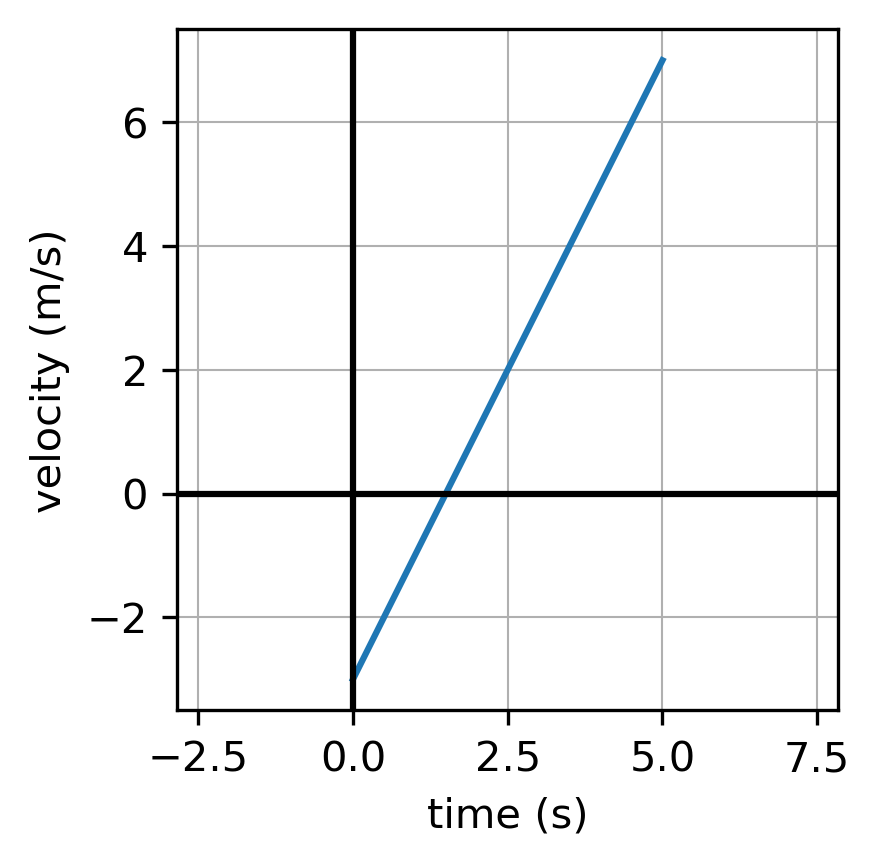
\includegraphics[]{week4-v1-t.png}

\item The following plot shows constant acceleration over time. If the initial velocity is $v_i=\SI{5}{m/s}$, then sketch a graph of velocity vs. time. \\
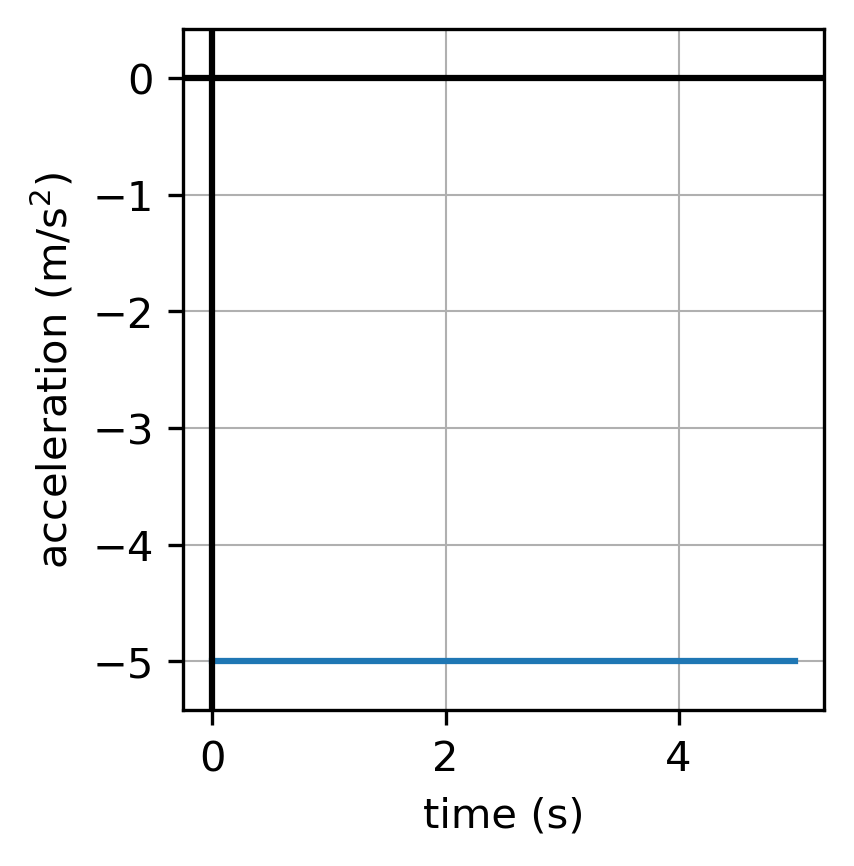
\includegraphics[]{week4-a1-t.png} 

\item The following plot shows the position of an object over time. What is the sign of the acceleration? What is the sign of the initial velocity? Approximately when does the object come to a stop?\\
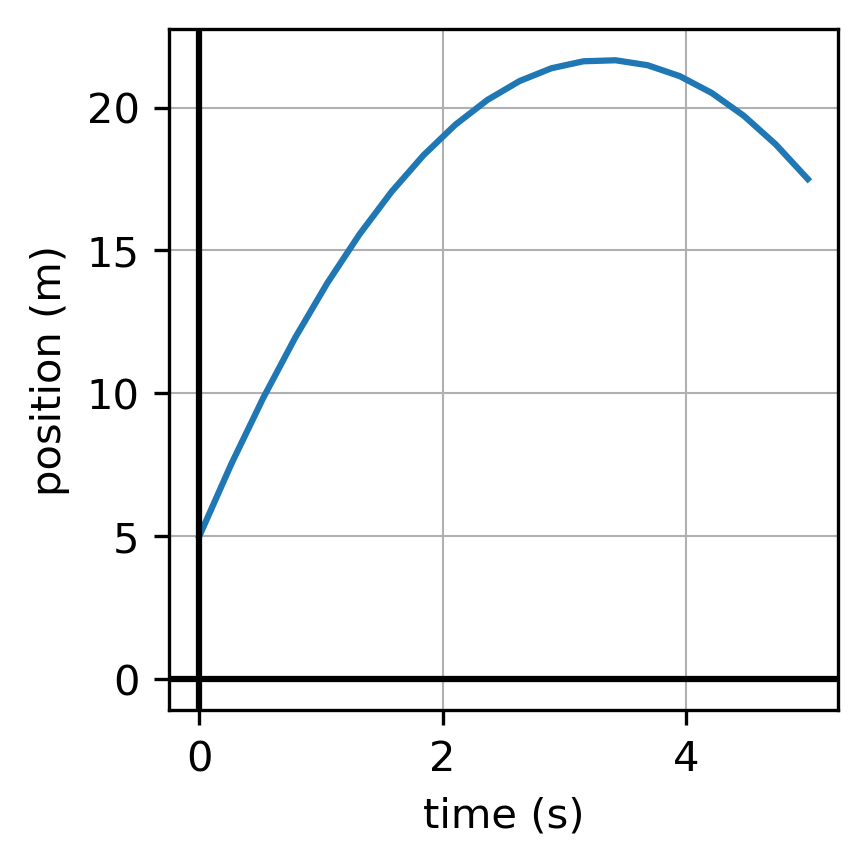
\includegraphics[]{week4-x1-t.png}

\item
A turtle starts walking in a straight line at a steady speed from a position $x=\SI{2.1}{\meter}$ to a position of $x=\SI{5.4}{\meter}$ in 10 seconds. Draw a plot of position vs time for this motion. Draw a plot of velocity vs. time for this motion. Label all the important features on these graphs.

\item
Draw a plot of velocity vs time for a case of 0 acceleration. Positive acceleration? Negative acceleration?

\item 
Draw a plot of velocity vs time for an object that is initially moving forward, but then stops and starts to move backward. Assume constant acceleration. What is the sign of the acceleration and what does that mean for the slope of this plot?\bigskip

\item What does a plot of position vs time look like for the same case as before (initially moving forward, but then stopping and moving backward)?\bigskip

\item Since $g=\SI{9.8}{\newton/\kilogram}$ also happens to correspond to acceleration due to gravity when no other forces are acting on the object, many people say $g=\SI{9.8}{\meter/\second^2}$. What is $g$ in \si{feet/second^2}?

\item A \SI{1}{kg} object slides down a friction-less inclined plane. The plane has an incline angle of \ang{15}. What is the acceleration of the object? How far does the object gone down the plane in \SI{3}{seconds}?\bigskip

\item A \SI{1}{kg} object slides down a friction-less inclined plane. The \emph{length of the plane} is \SI{1}{\meter}, and the \emph{height above the horizontal} is \SI{10}{\centi\meter}. How long does it take the object to reach the bottom and how fast it is going when it gets there?\bigskip

\clearpage
\item Examples 4.1, 4.2 and 4.3 from the text book (pgs. 127-130) are excellent and you should use the space below to work those out for yourself.
\clearpage

\item Here is an example of turning a problem inside out. In the lecture video, I worked an example of a person throwing an object up and off the edge of a bridge. The object goes up and then comes down and splashes in the water below, \SI{44.1}{\meter} below the place where it was released. In the example, we knew the time and found the initial velocity to be \SI{+8.66}{\meter / \second}. In this problem, use this information to find the time. (You should get \SI{4}{seconds})

\item I am standing at the very edge of a cliff and I want to know how far down it is to the ground or the water below me. To do this, I drop a rock off the edge, and count how long it takes to hit the ground. What is a general expression for the height of the cliff based on the amount of time it takes to hit the ground? If it takes \SI{4}{seconds} to do this, how high is the cliff? 

\item What is the velocity of a ball when it reaches its highest height after being thrown straight up?
\item What is the acceleration of a ball when it reaches its highest height after being thrown straight up?
\item If I throw a ball upward, what is an expression for the amount of time it takes to reach its highest height? If the initial velocity is \SI{15}{m/s}, then how much time does it take? 
\item How much time does it take for the ball thrown straight up to come back down?
\item So if I throw a ball straight up and its total travel time from when it leaves my hand to when it comes back down is \SI{4}{seconds}, then what was the original speed with which I threw it?
\item What is the final speed when the ball in the previous problem comes back down? (Assume final position is the same height from which I threw it.)




\item The moon has a gravitational field strength $g=\SI{1.6}{N/kg}$, so objects feel lighter on the moon in terms of lifting them vertically, but what about pushing horizontally? If you wanted to accelerate an \SI{10}{kg} object horizontally (on a frictionless surface) on the moon with an acceleration of \SI{2}{\meter/\second^2} , what force would you need to provide? Would this force be different on the earth? Why?

\item I am pushing a \SI{200}{\kilogram} box across a friction-full surface with \SI{750}{\newton} force. The coefficient of friction between the box and the floor is $\mu=0.5$. What is the net force on the box? What is the acceleration? What does the sign mean here? If the box was moving at \SI{3}{m/s} when I began to encounter the friction patch on the floor, how long does it take to come to a stop?\bigskip

\item I give a \SI{2}{kg} book a quick push to start it sliding across a table at \SI{10}{m/s} initially after my push it done, and it slides about \SI{1}{m} across the table before it comes to a stop, then what is the coefficient of friction between the book and table?\bigskip

\subsubsection*{The next two problems are here to set up the lab next week and are more in the vein of last week's problems, but still apply and are good to work through.}\vspace{-1in}

\item I am pulling two objects connected by a string. They are both \SI{100}{\kilogram}. There is no friction between the objects and the surface, and they are accelerating at \SI{1}{\meter/\second^2}. What is my pulling force and what tension force is between the strings?

\item One object $m_1$ connected by a string to another object $m_2$ that is hanging off the edge of the table. There is a pulley at the edge of the table so the string is not introducing any friction to the system. If this is a friction-less table, then what is an expression for the acceleration of the objects?

\item Now do the previous problem again, but with a coefficient of friction $\mu$ between the sliding mass ($m_1$) and the surface.



\end{enumerate}